% !TeX encoding = UTF-8

\chapter{ANÁLISE DOS RESULTADOS}\label{ch:resultados}
Este capítulo tem como finalidade apresentar os resultados obtidos através das implementações demonstradas no Capítulo 5.

\section{ANÁLISE DAS SÉRIES UTILIZADAS}
Após a implementação do modelo da RNA, através dos conjuntos de dados coletados, faz-se necessário avaliar como a respectiva técnica se comportou. Tendo isso em vista, a mesma foi aplicada em função do objetivo principal do trabalho, que é medir a capacidade de precisão de acerto no valor de abertura das ações. Portanto nas seções posteriores foi elaborada, de forma independente, uma análise de eficácia do modelo para o cenário de cada empresa utilizada no presente trabalho. É importante ressaltar que os modelos foram implementados levando em consideração todos os \textit{scripts}, métodos e ferramentas utilizadas no capítulo anterior.

\subsection{Análise do modelo da RNA: Intel Corporation}
A rede da Intel Corporation foi treinada com o objetivo de capturar o maior nível de variação possível dos dados, visando mapear um maior conjunto de padrões e, assim, responder de forma eficiente à dados dispersos através de uma boa capacidade de generalização. Tendo isso em vista, o período de treinamento preparado foi de 09/04/2001 até 21/08/2017.

Para o presente caso foram construídos dois cenários de simulação, buscando capacitar a rede à utilizar um parâmetro de ciclos de treinamento adequado ao modelo de dados utilizado. As métricas definidas para análise, a partir destes ciclos de treinamento, são: o comportamento da função de custo que compõem o modelo (erro quadrático médio, EQM) e a margem de erro dos valores resultantes da rede no período de 23/08/2017 a 31/08/2017 em relação aos valores reais. Os parâmetros utilizados foram: 200 e 1000 iterações.

\subsubsection{Intel Corporation: Treinamento com 200 Iterações}	
A ideia de executar o treinamento com uma quantidade baixa de iterações, é feita com o intuito de proporcionar um treinamento mais rápido com resultados significativos, levando em consideração as características especificas do modelo de dados. Assim, a configuração de treinamento da rede foi de 200 iterações x 4117 linhas, onde as linhas são a quantidade de registros do período de testes. Portanto, o modelo foi exposto a calculado por um total de 823.400 exemplos. O Gráfico 8 demonstra, de acordo com a quantidade de ciclos, a variação do EQM.
\begin{grafico}[h]
	\centering
	\fbox{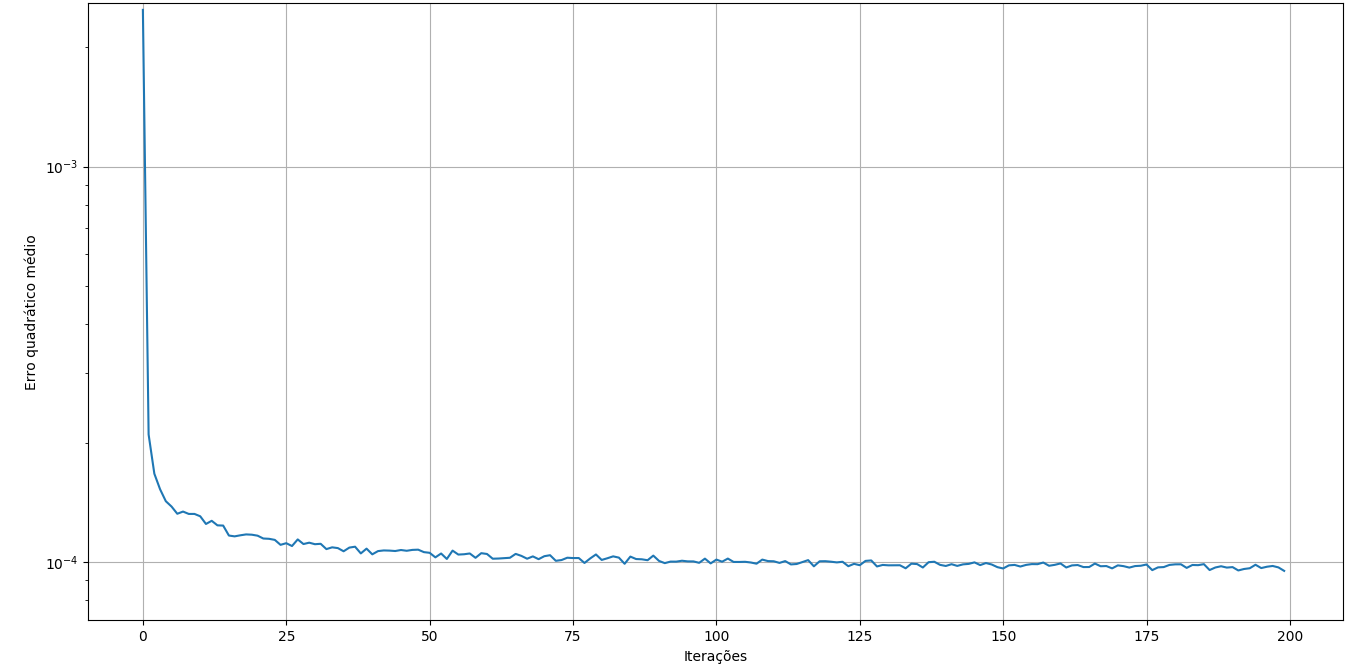
\includegraphics[width=1\textwidth]{erro_intel_comgrid}}
	\caption{Decaimento do EQM no treinamento da rede}
	\fonte{Elaborado pelo autor}
	\label{lingua}
\end{grafico}

O Gráfico 8 ilustra a variação dos resultados obtidos. O EQM iniciou-se, na primeira iteração, com um erro percentual de 0.00248996652176 e, após o término das 200 épocas de treinamento, concluí-se com um erro percentual de 9.49359025338.$10^{-05}$.

Analisando o gráfico, pode-se observar que o erro obteve uma queda brusca nas primeiras 75 iterações, enquanto que, nas 125 iterações posteriores, manteve o padrão com valores aproximados. A queda brusca e rápida do valor está diretamente ligada ao modelo de dados utilizado. Como detalhado na Seção 5.1, as ações da Intel não sofrem grande variabilidade no período coletado, tornando-se assim mais rápida de ser abstraída pela RNA.

Já o período destinado à testes, especificado na Seção 6.1.1, é exposto de na Tabela 1, detalhando quais foram os valores aplicados.
\begin{table}[h]
\centering
\caption{Período dos dados utilizados para testes: Intel Corporation}
\vspace{0.5cm}
\begin{tabular}{>{\centering\arraybackslash}m{2cm} >{\centering\arraybackslash}m{2cm} >{\centering\arraybackslash}m{2cm} >{\centering\arraybackslash}m{2cm} >{\centering\arraybackslash}m{2cm} >{\centering\arraybackslash}m{2cm}}
\toprule
Data    & Abertura   & Alta   & Baixa   & Fechamento   & Volume\\
\midrule
23/08/2017 & 34.54 & 34.81 & 34.38 & 34.66 & 196.481,34\\
24/08/2017 & 34.70 & 34.89 & 34.55 & 34.71 & 143.018,92\\
25/08/2017 & 34.82 & 34.93 & 34.58 & 34.67 & 147.268,29\\
28/08/2017 & 34.78 & 34.80 & 34.59 & 34.65 & 207.128,76\\
29/08/2017 & 34.51 & 34.75 & 34.46 & 34.73 & 158.436,68\\
30/08/2017 & 34.75 & 34.96 & 34.63 & 34.89 & 185.650,07\\
31/08/2017 & 34.94 & 35.18 & 34.87 & 35.07 & 163.667,72\\
\bottomrule
\end{tabular}
\end{table}

Os dados demonstrados na Tabela 1 foram refinados e normalizados de acordo com os métodos implementados no Capítulo 5. Após a execução deste processo, os mesmos foram inseridos na RNA para ativação. Posteriormente, foi realizada a desnormalização e os resultados apresentados. A Tabela 2 ilustra os resultados obtidos.
\begin{table}[h]
\centering
\caption{Resultados da predição realizada nos dados utilizados pela rede}
\vspace{0.5cm}
\begin{tabular}{>{\centering\arraybackslash}m{3cm} >{\centering\arraybackslash}m{3cm} >{\centering\arraybackslash}m{3cm} >{\centering\arraybackslash}m{3cm}}
\toprule
Data    & Valor esperado   & Resultado    & Erro (\%)\\
\midrule
23/08/2017 & 34.54 & 34.73 & 0.550\\
24/08/2017 & 34.70 & 34.71 & 0.028\\
25/08/2017 & 34.82 & 34.79 & 0.086\\
28/08/2017 & 34.78 & 34.77 & 0.028\\
29/08/2017 & 34.51 & 34.75 & 0.695\\
30/08/2017 & 34.75 & 34.82 & 0.201\\
31/08/2017 & 34.94 & 34.99 & 0.143\\
\bottomrule
\end{tabular}
\end{table}

Analisando a Tabela 2, pode-se observar que os resultados obtidos foram significativos, onde o percentual de erro calculado, através do erro relativo percentual, não ultrapassou a margem 0.70\%, se aproximando consideravelmente dos valores reais. A média de todo o período analisado obteve um erro de 0.20\%. O Gráfico 9 representa, de maneira ilustrativa, os resultados da série.
\begin{grafico}[h]
	\centering
	\fbox{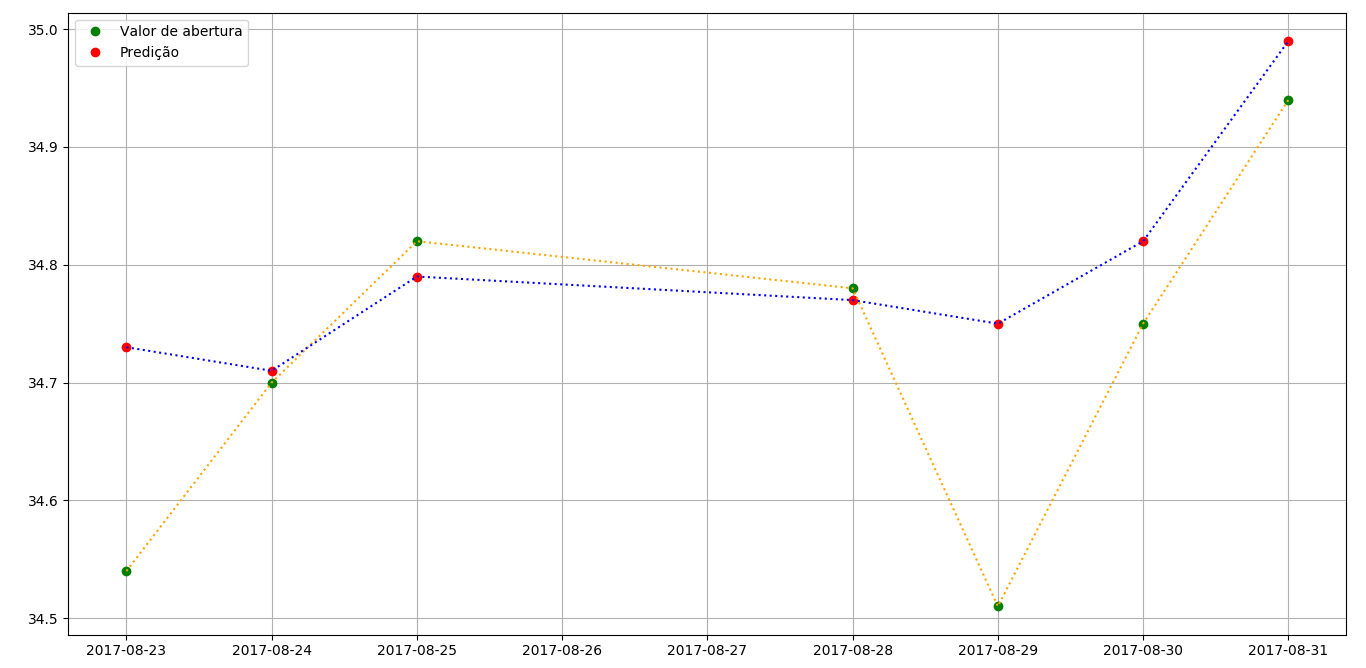
\includegraphics[width=1\textwidth]{predicao_intel}}
	\caption{Distribuição dos dados resultantes da RNA e seus valores esperados}
	\fonte{Elaborado pelo autor}
	\label{lingua}
\end{grafico}

Pelo gráfico também é possível observar como os resultados são próximos aos esperados. Os valores de abertura, nos respectivos dias testados, são representados por um ponto verde. Já os resultados obtidos pela rede são caracterizados pelo ponto vermelho. 

\subsubsection{Intel Corporation: Treinamento com 1000 Iterações}	
